\documentclass[a4paper,twoside,12pt]{article}
\usepackage[top=1.5cm,left=1.5cm,right=1.5cm,bottom=2cm]{geometry}

\usepackage[utf8]{inputenc}
\usepackage[T1]{fontenc}
\usepackage{lmodern}
\usepackage[brazilian]{babel}

\usepackage{graphicx}
\usepackage{subfig}
\usepackage{psfrag}
\usepackage{cite}
\usepackage[cmex10]{amsmath}
\usepackage{amssymb}
\usepackage{upgreek}
\usepackage{microtype}
\usepackage{titling}
\usepackage{courier}
\usepackage{url}
\usepackage{hyperref}
\hypersetup{
	colorlinks=true,
	linkcolor=blue,
	urlcolor=blue
}

% Use o pacote 'listings' para adicionar código e o pacote 'color' para gerar os destaques
\usepackage{listings}
\usepackage{color}
\definecolor{grey}{rgb}{0.6,0.6,0.6}
\definecolor{codegreen}{rgb}{0,0.6,0}
\definecolor{codegray}{rgb}{0.5,0.5,0.5}
\definecolor{codepurple}{rgb}{0.58,0,0.82}
\definecolor{backcolour}{rgb}{0.95,0.95,0.92}
\lstset{language=Python,				% definir para destaque de linguagem Python
	backgroundcolor=\color{backcolour},
	commentstyle=\color{codegreen},
	keywordstyle=\color{magenta},
	numberstyle=\tiny\color{codegray},
	stringstyle=\color{codepurple},
	basicstyle=\ttfamily\small,		% definir tamanho das fontes
	breaklines=true,				% definir quebra de linha automática
	linewidth=\textwidth,			% definir tamanho da caixa de código
	showstringspaces=false}			% mostrar espaços como sublinhados apenas dentro de strings


\title{\vspace{-2cm} Processamento Digital de Sinais\\ Soluções para Tutorial 14 - Sistemas tipo Atraso e Reflexões Acústicas}
\author{\url{https://github.com/fchirono/Aulas_PDS_Acustica}}

\begin{document}
	\date{}
	\maketitle
	
	
	\setcounter{section}{1}
	\section{Tarefas}
	
	\subsection{Resposta ao Impulso de um Sistema Atraso Ideal}
	
	\subsubsection*{Tarefa 1}
	
	A função abaixo implementa as duas abordagens solicitadas, ambas \emph{exatas}. No domínio do tempo (\texttt{'t'}), calcula-se diretamente a função $\mathrm{sinc}(n-n_0)$ centrada na amostra de atraso $n_0 = T_{atraso}\,f_s$ (possivelmente fracionária). No domínio da frequência (\texttt{'f'}), constrói-se o termo de fase linear $e^{-j2\pi f T_0}$ usando o vetor de frequências \emph{bilateral} retornado por \texttt{numpy.fft.fftfreq}, e aplica-se a IFFT para obter a resposta ao impulso.
	
	\begin{lstlisting}[frame=single]
import numpy as np

def cria_impulso_atrasado(T_atraso, T_duracao, fs, t_ou_f='f'):
    """
    Funcao para criar um sinal tipo impulso atrasado com amplitude unitaria e 
    atraso 'T_atraso' (em segundos), e frequencia de amostragem 'fs'. O calculo
    pode ser realizado no dominio do tempo ou da frequencia.

    Parametros
    ----------
    T_atraso : float
        Atraso do impulso, em segundos.

    T_duracao : float
        Duracao do sinal, em segundos.

    fs : float
        Frequencia de amostragem, em Hz.

    t_ou_f : {"t", "f"}
        Flag indicando se o calculo sera realizado no dominio do tempo ("t") 
        usando uma funcao sinc, ou da frequencia ("f") usando atraso de fase.
        O valor padrao eh "f".

    Retorna
    -------
    t : (N,)-array
        Vetor de amostras no tempo, em segundos

    impulso : (N,)-array
        Sinal tipo impulso atrasado, em amostras
    """

    # intervalo de amostragem (segundos)
    dt = 1/fs

    # numero total de amostras no sinal
    N_amostras  = int(T_duracao*fs)

    # vetor de amostras no tempo
    t = np.linspace(0, T_duracao-dt, N_amostras)

    if t_ou_f == "t":

        # a resposta ao impulso ideal eh uma funcao sinc centrado em 'n_atraso'
        nt = np.arange(N_amostras)
        n_atraso = T_atraso/dt
        impulso = np.sinc(nt - n_atraso)

    elif t_ou_f == "f":

        # cria vetor de frequencias com 'N_amostras', contendo frequencias
        # positivas (0 a fs/2) e negativas (-fs/2 a 0)
        f = np.fft.fftfreq(N_amostras, dt)

        # Calcula um atraso na frequencia
        Xf = np.exp(-1j * 2*np.pi * f * T_atraso)

        # Usa a IFFT para calcular a Resposta ao Impulso do sinal atraso
        impulso = np.fft.ifft(Xf, n=N_amostras)

    return t, impulso.real
	\end{lstlisting}
	
	\textbf{Nota importante}: se um vetor de frequências estritamente positivas (\texttt{np.linspace(0, fs, N)}, por exemplo) for usado no lugar de \texttt{np.fft.fftfreq}, o termo de fase $e^{-j2\pi f T_0}$ deixará de representar corretamente um atraso real quando $T_0$ é fracionário, e a IFFT resultante apresentará artefatos: a RI deixa de ser puramente real, ou apresenta oscilações espúrias. Isso ocorre porque a simetria conjugada do espectro de um sinal real ($X(-f) = X^*(f)$) só é respeitada quando as frequências negativas são explicitamente incluídas no cálculo.
	
	\subsubsection*{Tarefas 2 e 3}
	
	A Figura \ref{fig:T1_int} compara, com um ``zoom'' em torno da amostra de atraso, as RIs obtidas pelas duas implementações para um atraso \emph{inteiro} de $n_0=1253$ amostras ($f_s=48\,000$ Hz), sobrepostas à função $\mathrm{sinc}(n-n_0)$ de referência (amostrada a $100 f_s$ para aproximar a curva ``contínua''). As três curvas coincidem ponto a ponto: um único pico unitário em $n=1253$, e valor exatamente nulo em todas as demais amostras inteiras -- pois $\sin[\pi(n-n_0)]=0$ sempre que $n-n_0$ é um inteiro não-nulo. Como esperado, a curva ``contínua'' também passa pelos cruzamentos de zero exatamente nos instantes de amostragem, de modo que a discretização recupera, neste caso, o impulso discreto ideal $h[n]=\delta[n-n_0]$.
	
	\begin{figure}[h!]
		\centering
		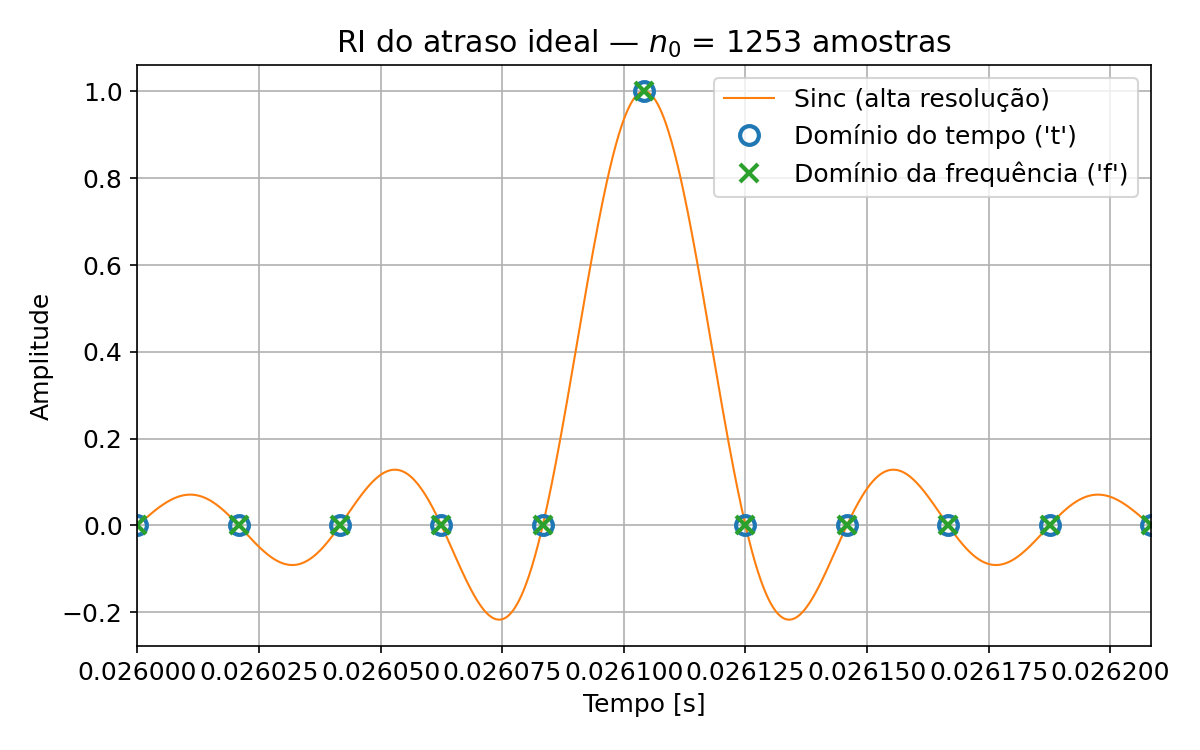
\includegraphics[width = 0.7\textwidth]{T1_RI_inteiro.png}
		\caption{RI de um atraso ideal de $n_0=1253$ amostras (inteiro), calculada nos domínios do tempo e da frequência, e comparada com a função $\mathrm{sinc}(n-n_0)$ de referência (curva contínua, amostrada a $100f_s$).}
		\label{fig:T1_int}
	\end{figure}
	
	\subsubsection*{Tarefa 4}
	
	Repetindo o procedimento para um atraso \emph{fracionário} de $n_0=1253.45$ amostras, a Figura \ref{fig:T1_frac} mostra que as três curvas continuam coincidindo exatamente -- mas agora nenhuma amostra discreta cai sobre o pico da sinc (que ocorre em $n=1253.45$, entre duas amostras). Note que o valor máximo amostrado é $\approx 0.7$, ou seja, abaixo de 1. Note também que a RI deixa de ser um impulso discreto e passa a ser uma sequência que se ``espalha'' por toda a duração do sinal, de $n=-\infty$ a $+\infty$.
	
	\begin{figure}[h!]
		\centering
		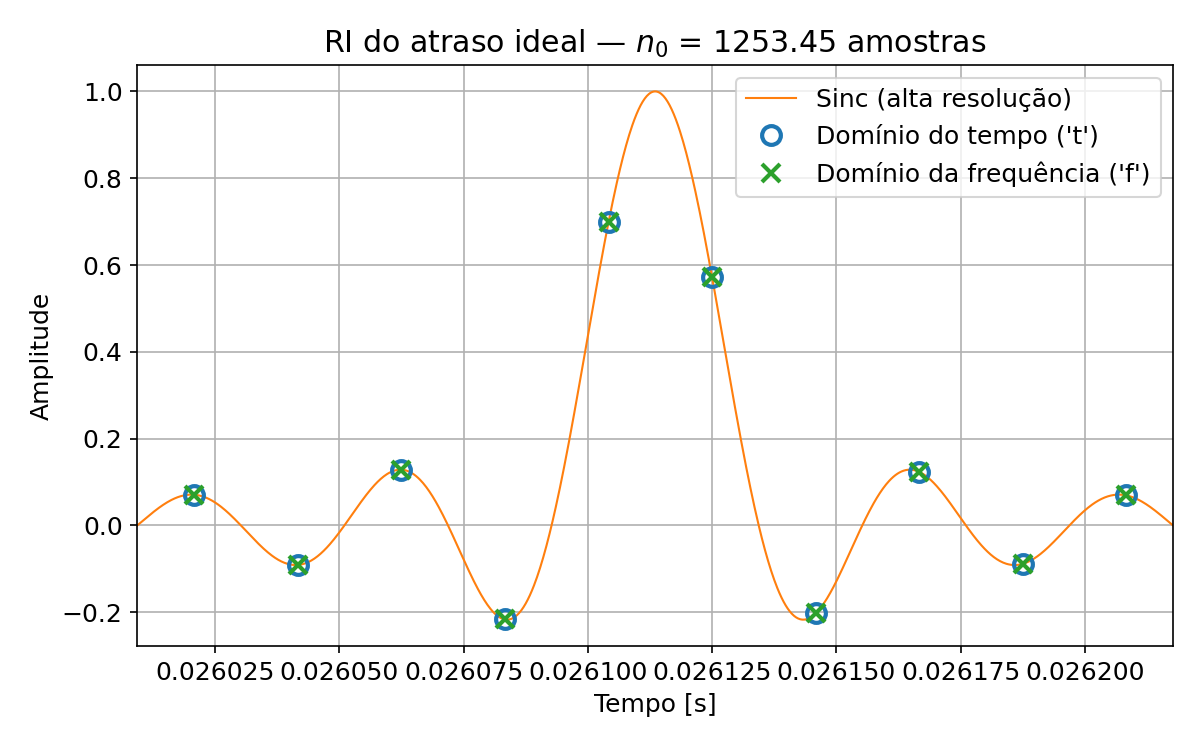
\includegraphics[width = 0.7\textwidth]{T1_RI_fracionario.png}
		\caption{RI de um atraso ideal de $n_0=1253.45$ amostras (fracionário), calculada nos domínios do tempo e da frequência, e comparada com a função $\mathrm{sinc}(n-n_0)$ de referência (curva contínua, amostrada a $100f_s$).}
		\label{fig:T1_frac}
	\end{figure}
	
	As duas implementações são matematicamente equivalentes, tanto para atrasos inteiros quanto fracionários: calcular $\mathrm{sinc}(n-n_0)$ diretamente no tempo, ou multiplicar o espectro por $e^{-j\Omega T_0}$ e aplicar a IFFT, são apenas duas formas diferentes de obter a \emph{mesma} resposta ao impulso teórica.
	\newpage
	\subsection{Sistema Fonte-Parede-Receptor}
	
	\subsubsection*{Tarefa 1: Resposta ao Impulso analítica}
	
	Pelo método das imagens (Seção 1.2 do enunciado), o receptor recebe a superposição de duas ondas acústicas: o som direto, vindo da fonte real a uma distância $D_{FR}$, e o som refletido, equivalente ao som advindo de uma fonte imagem a uma distância $D_{eco} = \sqrt{D_{FR}^2 + (2D_{FP})^2}$. Assumindo uma parede rígida (reflexão sem perda de energia nem inversão de fase), a resposta ao impulso do sistema é a soma das duas respostas individuais:
	\begin{equation}
		\boxed{h(t) = \frac{1}{D_{FR}} \, \delta\!\left(t - \frac{D_{FR}}{c_0}\right) \; + \; \frac{1}{D_{eco}} \, \delta\!\left(t - \frac{D_{eco}}{c_0}\right)}.
	\end{equation}
	
	\subsubsection*{Tarefa 2: Resposta em Frequência analítica}
	
	Aplicando a Transformada de Fourier ao resultado da Tarefa 1 (par $\delta(t-T) \leftrightarrow e^{-j2\pi f T}$):
	\begin{equation}
		\boxed{H(f) = \frac{1}{D_{FR}} \, e^{-j 2\pi f T_1} \; + \; \frac{1}{D_{eco}} \, e^{-j 2\pi f T_2}}, \qquad T_1 = \frac{D_{FR}}{c_0}, \quad T_2 = \frac{D_{eco}}{c_0}.
	\end{equation}
	
	\subsubsection*{Tarefa 3: Oscilação senoidal de $|H(f)|^2$}
	
	Escrevendo $A_1 = 1/D_{FR}$ e $A_2 = 1/D_{eco}$ para simplificar a notação, temos $H(f) = A_1 e^{-j2\pi f T_1} + A_2 e^{-j2\pi f T_2}$. A magnitude ao quadrado é:
	\begin{align}
		|H(f)|^2 &= H(f)\, H^*(f) \nonumber \\
		&= \left(A_1 e^{-j2\pi f T_1} + A_2 e^{-j2\pi f T_2}\right)\left(A_1 e^{j2\pi f T_1} + A_2 e^{j2\pi f T_2}\right) \nonumber \\
		&= A_1^2 + A_2^2 + A_1 A_2 \left[e^{-j2\pi f(T_1-T_2)} + e^{j2\pi f(T_1-T_2)}\right] \nonumber \\
		&= A_1^2 + A_2^2 + 2 A_1 A_2 \cos\!\big[2\pi f (T_2-T_1)\big].
	\end{align}
	
	Ou seja:
	\begin{equation}
		\boxed{|H(f)|^2 = \frac{1}{D_{FR}^2} + \frac{1}{D_{eco}^2} + \frac{2}{D_{FR}D_{eco}} \cos\!\big[2\pi f \, \Delta T\big]}, \qquad \Delta T = T_2 - T_1 = \frac{D_{eco}-D_{FR}}{c_0}.
	\end{equation}
	
	Esta expressão é a soma de um termo constante ($A_1^2+A_2^2$, o ``piso'' médio) com um termo puramente \textbf{senoidal em $f$}, de amplitude $2A_1A_2$ e frequência angular $2\pi \Delta T$ (rad por Hz). Como o cosseno tem período $2\pi$ em seu argumento, o período de oscilação de $|H(f)|^2$ \emph{ao longo do eixo de frequências} -- isto é, o espaçamento $\Delta f$ entre picos (ou vales) consecutivos -- é obtido fazendo $2\pi \Delta f \, \Delta T = 2\pi$:
	\begin{equation}
		\boxed{\Delta f = \frac{1}{\Delta T} = \frac{c_0}{D_{eco}-D_{FR}}}.
	\end{equation}
	
	Este é exatamente o padrão de \textbf{filtro-pente} (\emph{comb filter}) característico da interferência entre um sinal direto e uma única reflexão: quanto \emph{menor} a diferença de caminho $D_{eco}-D_{FR}$ (i.e., quanto mais próximas as duas distâncias percorridas), \emph{maior} o espaçamento em frequência entre os ``dentes'' do pente; e quanto \emph{maior} a diferença de caminho, mais estreitos (mais próximos entre si) ficam os vales de cancelamento.
	
	\subsubsection*{Tarefa 4: Verificação numérica}
	
	Para $D_{FR}=1$ m, $D_{FP}=0.5$ m e $c_0=340$ m/s, obtemos $D_{eco} = \sqrt{1^2+(2\cdot0.5)^2} = \sqrt{2} \approx 1.414$ m, $T_1 \approx 2.94$ ms, $T_2 \approx 4.16$ ms, e portanto:
	\begin{equation}
		\Delta T = T_2-T_1 \approx 1.22 \text{ ms} \quad \Longrightarrow \quad \Delta f = \frac{1}{\Delta T} \approx 820.8 \text{ Hz}.
	\end{equation}
	
	A Figura \ref{fig:T2_RI} mostra a resposta ao impulso numérica (calculada com a função \texttt{cria\_impulso\_atrasado} no modo \texttt{'f'}), com os dois impulsos localizados exatamente em $T_1$ e $T_2$, com amplitudes nominais $1/D_{FR}=1$ e $1/D_{eco}\approx0.707$, respectivamente. Como ambos os atrasos são fracionários (ver Tarefa 1.4), cada impulso é, na verdade, uma sinc espalhada em torno de sua amostra central; portanto, os picos numéricos observados ($\approx 0.95$ e $\approx 0.58$) se afastam um pouco dos valores nominais $1$ e $0.707$.
	
	\begin{figure}[h!]
		\centering
		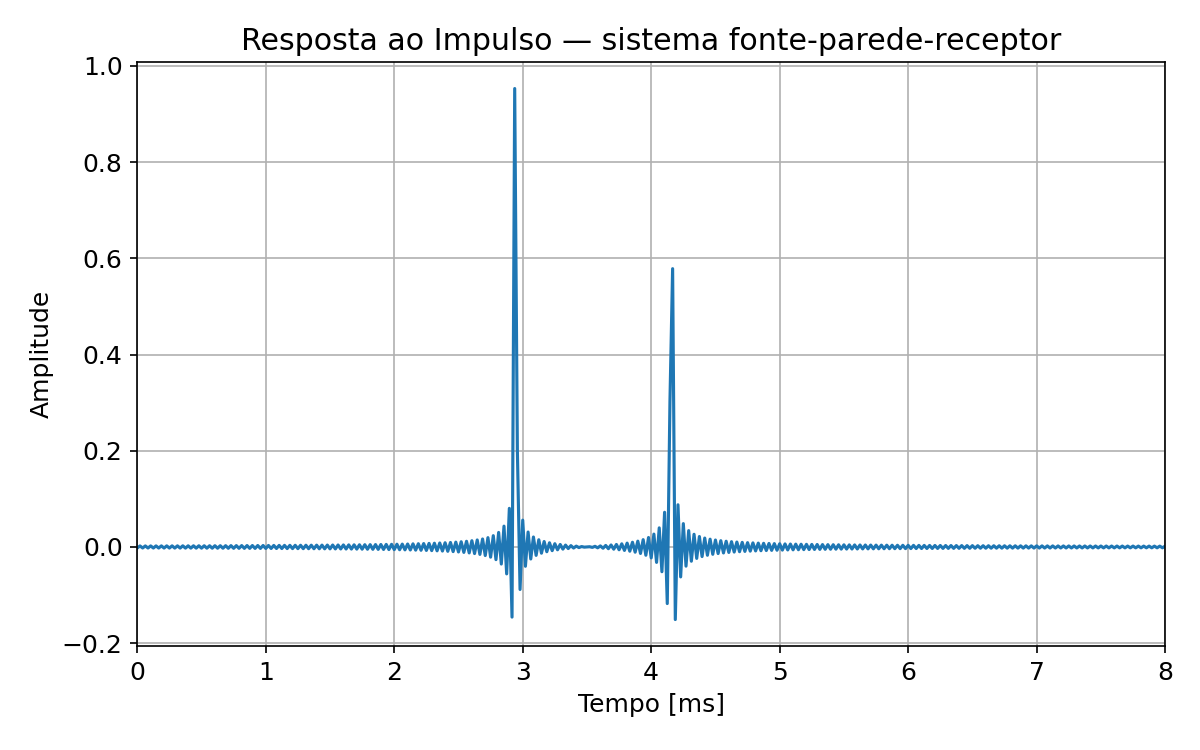
\includegraphics[width = 0.7\textwidth]{T2_RI_eco.png}
		\caption{Resposta ao impulso numérica do sistema fonte-parede-receptor, para $D_{FR}=1$ m e $D_{FP}=0.5$ m.}
		\label{fig:T2_RI}
	\end{figure}
	
	A Figura \ref{fig:T2_RF} mostra $|H(f)|^2$ obtida pela FFT da RI numérica. O padrão de filtro-pente é claramente visível, com picos e vales espaçados por aproximadamente $821$ Hz, em excelente concordância com o valor previsto na Tarefa 3.
	
	\begin{figure}[h!]
		\centering
		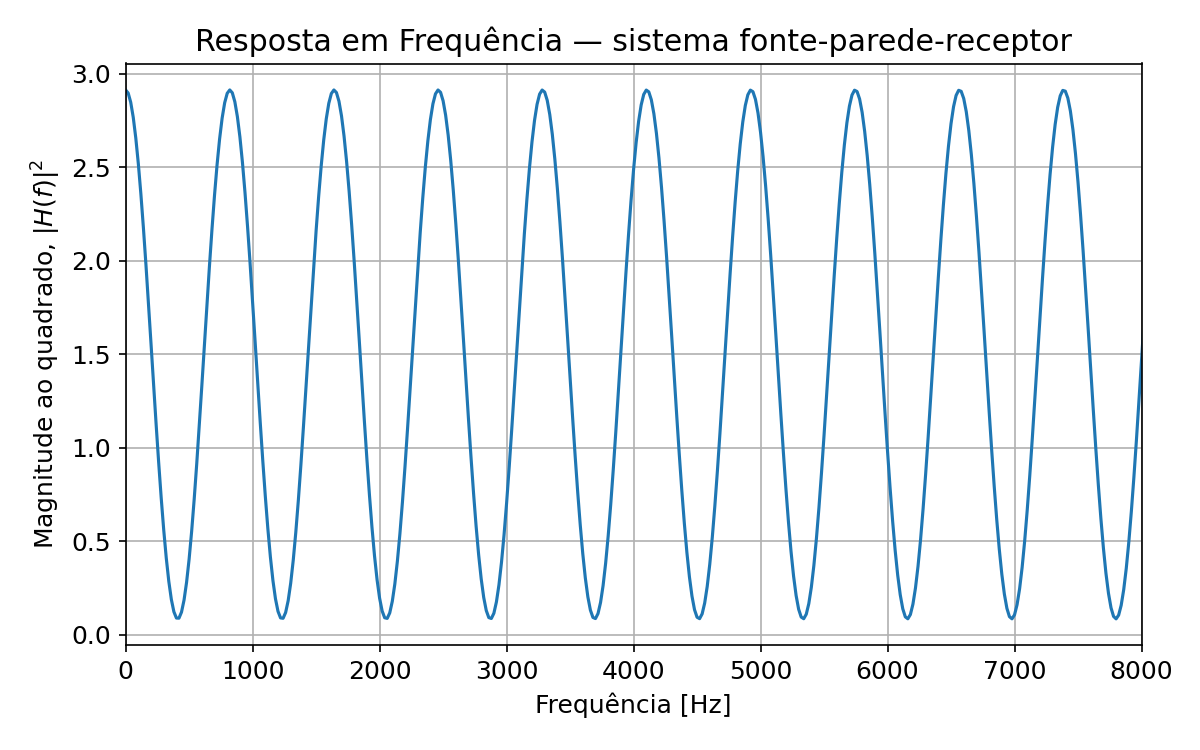
\includegraphics[width = 0.7\textwidth]{T2_RF_eco.png}
		\caption{Resposta em frequência (magnitude ao quadrado) do sistema fonte-parede-receptor, para $D_{FR}=1$ m e $D_{FP}=0.5$ m. O espaçamento entre picos (ou vales) consecutivos é de aproximadamente $\Delta f \approx 821$ Hz, conforme previsto analiticamente.}
		\label{fig:T2_RF}
	\end{figure}
	
	\subsubsection*{Tarefa 5: Auralização}
	
	A convolução da resposta ao impulso $h[n]$ com um sinal de ruído branco (ou uma gravação de voz) simula o efeito acústico da reflexão sobre o sinal original.	Como o atraso entre o som direto e o refletido ($\approx 1.22$ ms, neste exemplo) é bem abaixo do limiar de percepção de eco distinto -- tipicamente $\geq$ 30-50 ms para sinais de fala -- o ouvido humano \textbf{não} percebe as duas chegadas como sons separados (um ``eco''), mas sim como uma única fonte sonora com \textbf{timbre alterado}: o filtro-pente resultante atenua e reforça periodicamente diferentes bandas de frequência (com vales a cada $\sim$821 Hz), produzindo uma coloração espectral característica, muitas vezes descrita como um som mais ``metálico'', ``oco'' ou ``nasal'' em comparação com o som direto sem a reflexão. Para geometrias com maior diferença de caminho $D_{eco}-D_{FR}$ (atrasos maiores que $\sim$30-50 ms), este mesmo sistema passaria a ser percebido como um eco distinto, em vez de uma simples coloração timbral -- este seria, por exemplo, o caso de uma reflexão em uma parede bem mais afastada da linha fonte-receptor.
	
\end{document}